\documentclass[twoside]{book}

% Packages required by doxygen
\usepackage{calc}
\usepackage{doxygen}
\usepackage{graphicx}
\usepackage[utf8]{inputenc}
\usepackage{makeidx}
\usepackage{multicol}
\usepackage{multirow}
\usepackage{fixltx2e}
\PassOptionsToPackage{warn}{textcomp}
\usepackage{textcomp}
\usepackage[nointegrals]{wasysym}
\usepackage[table]{xcolor}

% Font selection
\usepackage[T1]{fontenc}
\usepackage{mathptmx}
\usepackage[scaled=.90]{helvet}
\usepackage{courier}
\usepackage{amssymb}
\usepackage{sectsty}
\renewcommand{\familydefault}{\sfdefault}
\allsectionsfont{%
  \fontseries{bc}\selectfont%
  \color{darkgray}%
}
\renewcommand{\DoxyLabelFont}{%
  \fontseries{bc}\selectfont%
  \color{darkgray}%
}
\newcommand{\+}{\discretionary{\mbox{\scriptsize$\hookleftarrow$}}{}{}}

% Page & text layout
\usepackage{geometry}
\geometry{%
  a4paper,%
  top=2.5cm,%
  bottom=2.5cm,%
  left=2.5cm,%
  right=2.5cm%
}
\tolerance=750
\hfuzz=15pt
\hbadness=750
\setlength{\emergencystretch}{15pt}
\setlength{\parindent}{0cm}
\setlength{\parskip}{0.2cm}
\makeatletter
\renewcommand{\paragraph}{%
  \@startsection{paragraph}{4}{0ex}{-1.0ex}{1.0ex}{%
    \normalfont\normalsize\bfseries\SS@parafont%
  }%
}
\renewcommand{\subparagraph}{%
  \@startsection{subparagraph}{5}{0ex}{-1.0ex}{1.0ex}{%
    \normalfont\normalsize\bfseries\SS@subparafont%
  }%
}
\makeatother

% Headers & footers
\usepackage{fancyhdr}
\pagestyle{fancyplain}
\fancyhead[LE]{\fancyplain{}{\bfseries\thepage}}
\fancyhead[CE]{\fancyplain{}{}}
\fancyhead[RE]{\fancyplain{}{\bfseries\leftmark}}
\fancyhead[LO]{\fancyplain{}{\bfseries\rightmark}}
\fancyhead[CO]{\fancyplain{}{}}
\fancyhead[RO]{\fancyplain{}{\bfseries\thepage}}
\fancyfoot[LE]{\fancyplain{}{}}
\fancyfoot[CE]{\fancyplain{}{}}
\fancyfoot[RE]{\fancyplain{}{\bfseries\scriptsize Generated on Thu May 8 2014 23\+:13\+:17 for My Project by Doxygen }}
\fancyfoot[LO]{\fancyplain{}{\bfseries\scriptsize Generated on Thu May 8 2014 23\+:13\+:17 for My Project by Doxygen }}
\fancyfoot[CO]{\fancyplain{}{}}
\fancyfoot[RO]{\fancyplain{}{}}
\renewcommand{\footrulewidth}{0.4pt}
\renewcommand{\chaptermark}[1]{%
  \markboth{#1}{}%
}
\renewcommand{\sectionmark}[1]{%
  \markright{\thesection\ #1}%
}

% Indices & bibliography
\usepackage{natbib}
\usepackage[titles]{tocloft}
\setcounter{tocdepth}{3}
\setcounter{secnumdepth}{5}
\makeindex

% Hyperlinks (required, but should be loaded last)
\usepackage{ifpdf}
\ifpdf
  \usepackage[pdftex,pagebackref=true]{hyperref}
\else
  \usepackage[ps2pdf,pagebackref=true]{hyperref}
\fi
\hypersetup{%
  colorlinks=true,%
  linkcolor=blue,%
  citecolor=blue,%
  unicode%
}

% Custom commands
\newcommand{\clearemptydoublepage}{%
  \newpage{\pagestyle{empty}\cleardoublepage}%
}


%===== C O N T E N T S =====

\begin{document}

% Titlepage & ToC
\hypersetup{pageanchor=false,
             bookmarks=true,
             bookmarksnumbered=true,
             pdfencoding=unicode
            }
\pagenumbering{roman}
\begin{titlepage}
\vspace*{7cm}
\begin{center}%
{\Large My Project }\\
\vspace*{1cm}
{\large Generated by Doxygen 1.8.7}\\
\vspace*{0.5cm}
{\small Thu May 8 2014 23:13:17}\\
\end{center}
\end{titlepage}
\clearemptydoublepage
\tableofcontents
\clearemptydoublepage
\pagenumbering{arabic}
\hypersetup{pageanchor=true}

%--- Begin generated contents ---
\chapter{Hierarchical Index}
\section{Class Hierarchy}
This inheritance list is sorted roughly, but not completely, alphabetically\+:\begin{DoxyCompactList}
\item \contentsline{section}{Map()}{\pageref{category_map_07_08}}{}
\item \contentsline{section}{Map$<$ Map\+Protocol $>$}{\pageref{interface_map}}{}
\item $<$Map\+Protocol$>$\begin{DoxyCompactList}
\item \contentsline{section}{Map}{\pageref{interface_map}}{}
\end{DoxyCompactList}
\item \contentsline{section}{Menu()}{\pageref{category_menu_07_08}}{}
\item \contentsline{section}{My\+Scene()}{\pageref{category_my_scene_07_08}}{}
\item N\+S\+Object\begin{DoxyCompactList}
\item \contentsline{section}{Game\+Settings}{\pageref{interface_game_settings}}{}
\item \contentsline{section}{Player}{\pageref{interface_player}}{}
\item \contentsline{section}{Player\+Positions}{\pageref{interface_player_positions}}{}
\end{DoxyCompactList}
\item \contentsline{section}{Player()}{\pageref{category_player_07_08}}{}
\item S\+K\+Node\begin{DoxyCompactList}
\item \contentsline{section}{Map}{\pageref{interface_map}}{}
\end{DoxyCompactList}
\item $<$S\+K\+Physics\+Contact\+Delegate$>$\begin{DoxyCompactList}
\item \contentsline{section}{My\+Scene}{\pageref{interface_my_scene}}{}
\end{DoxyCompactList}
\item S\+K\+Scene\begin{DoxyCompactList}
\item \contentsline{section}{Menu}{\pageref{interface_menu}}{}
\item \contentsline{section}{My\+Scene}{\pageref{interface_my_scene}}{}
\end{DoxyCompactList}
\item $<$U\+I\+Application\+Delegate$>$\begin{DoxyCompactList}
\item \contentsline{section}{App\+Delegate}{\pageref{interface_app_delegate}}{}
\end{DoxyCompactList}
\item U\+I\+Responder\begin{DoxyCompactList}
\item \contentsline{section}{App\+Delegate}{\pageref{interface_app_delegate}}{}
\end{DoxyCompactList}
\item U\+I\+View\+Controller\begin{DoxyCompactList}
\item \contentsline{section}{View\+Controller}{\pageref{interface_view_controller}}{}
\end{DoxyCompactList}
\item \contentsline{section}{View\+Controller()}{\pageref{category_view_controller_07_08}}{}
\end{DoxyCompactList}

\chapter{Class Index}
\section{Class List}
Here are the classes, structs, unions and interfaces with brief descriptions\+:\begin{DoxyCompactList}
\item\contentsline{section}{\hyperlink{interface_app_delegate}{App\+Delegate} }{\pageref{interface_app_delegate}}{}
\item\contentsline{section}{\hyperlink{interface_game_settings}{Game\+Settings} }{\pageref{interface_game_settings}}{}
\item\contentsline{section}{\hyperlink{interface_map}{Map} }{\pageref{interface_map}}{}
\item\contentsline{section}{\hyperlink{category_map_07_08}{Map()} }{\pageref{category_map_07_08}}{}
\item\contentsline{section}{\hyperlink{interface_menu}{Menu} }{\pageref{interface_menu}}{}
\item\contentsline{section}{\hyperlink{category_menu_07_08}{Menu()} }{\pageref{category_menu_07_08}}{}
\item\contentsline{section}{\hyperlink{interface_my_scene}{My\+Scene} }{\pageref{interface_my_scene}}{}
\item\contentsline{section}{\hyperlink{category_my_scene_07_08}{My\+Scene()} }{\pageref{category_my_scene_07_08}}{}
\item\contentsline{section}{\hyperlink{interface_player}{Player} }{\pageref{interface_player}}{}
\item\contentsline{section}{\hyperlink{category_player_07_08}{Player()} }{\pageref{category_player_07_08}}{}
\item\contentsline{section}{\hyperlink{interface_player_positions}{Player\+Positions} }{\pageref{interface_player_positions}}{}
\item\contentsline{section}{\hyperlink{interface_view_controller}{View\+Controller} }{\pageref{interface_view_controller}}{}
\item\contentsline{section}{\hyperlink{category_view_controller_07_08}{View\+Controller()} }{\pageref{category_view_controller_07_08}}{}
\end{DoxyCompactList}

\chapter{Class Documentation}
\hypertarget{interface_app_delegate}{\section{App\+Delegate Class Reference}
\label{interface_app_delegate}\index{App\+Delegate@{App\+Delegate}}
}
Inheritance diagram for App\+Delegate\+:\begin{figure}[H]
\begin{center}
\leavevmode
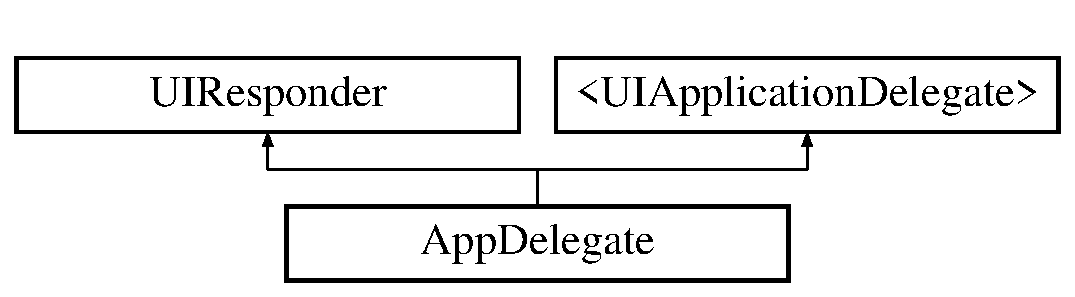
\includegraphics[height=2.000000cm]{interface_app_delegate}
\end{center}
\end{figure}
\subsection*{Properties}
\begin{DoxyCompactItemize}
\item 
\hypertarget{interface_app_delegate_acf48ac24125e688cac1a85445cd7fac2}{U\+I\+Window $\ast$ {\bfseries window}}\label{interface_app_delegate_acf48ac24125e688cac1a85445cd7fac2}

\end{DoxyCompactItemize}


The documentation for this class was generated from the following file\+:\begin{DoxyCompactItemize}
\item 
Centeye/App\+Delegate.\+h\end{DoxyCompactItemize}

\hypertarget{interface_game_settings}{\section{Game\+Settings Class Reference}
\label{interface_game_settings}\index{Game\+Settings@{Game\+Settings}}
}
Inheritance diagram for Game\+Settings\+:\begin{figure}[H]
\begin{center}
\leavevmode
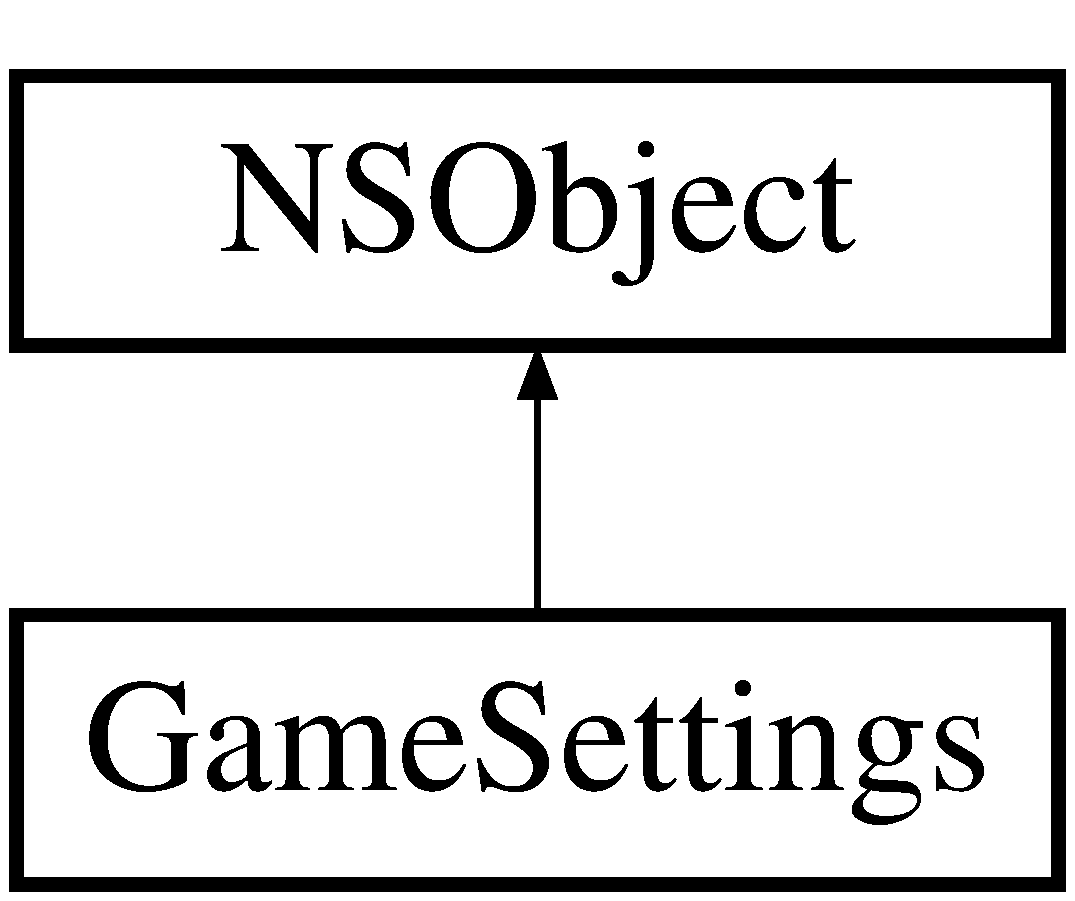
\includegraphics[height=2.000000cm]{interface_game_settings}
\end{center}
\end{figure}
\subsection*{Instance Methods}
\begin{DoxyCompactItemize}
\item 
\hypertarget{interface_game_settings_a50bb29b52dabe4f275e9758082189fbf}{(void) -\/ {\bfseries reset\+Defaults}}\label{interface_game_settings_a50bb29b52dabe4f275e9758082189fbf}

\item 
\hypertarget{interface_game_settings_a75a9177535614405dd026d997ba80c37}{(void) -\/ {\bfseries load\+User\+Defaults}}\label{interface_game_settings_a75a9177535614405dd026d997ba80c37}

\item 
\hypertarget{interface_game_settings_ae6bb2546dce1b78bb2b63f99b2086363}{(void) -\/ {\bfseries save\+User\+Defaults}}\label{interface_game_settings_ae6bb2546dce1b78bb2b63f99b2086363}

\end{DoxyCompactItemize}
\subsection*{Properties}
\begin{DoxyCompactItemize}
\item 
\hypertarget{interface_game_settings_a416a576c7d8af90c4d2184c46fcd88fe}{N\+S\+Integer {\bfseries number\+Of\+Players}}\label{interface_game_settings_a416a576c7d8af90c4d2184c46fcd88fe}

\item 
\hypertarget{interface_game_settings_a0aa6dff7097941bc44415ecb5621e929}{B\+O\+O\+L {\bfseries one\+By\+One}}\label{interface_game_settings_a0aa6dff7097941bc44415ecb5621e929}

\item 
\hypertarget{interface_game_settings_a4834e30796b43e263b411dbb715c4f22}{B\+O\+O\+L {\bfseries wait\+Until\+Still}}\label{interface_game_settings_a4834e30796b43e263b411dbb715c4f22}

\item 
\hypertarget{interface_game_settings_a10a3b35f1dbfb828a2ecb39108833551}{B\+O\+O\+L {\bfseries use\+Walls}}\label{interface_game_settings_a10a3b35f1dbfb828a2ecb39108833551}

\item 
\hypertarget{interface_game_settings_ad59e90cf13cbc22738be7eb191081df1}{B\+O\+O\+L {\bfseries use\+Size\+Up}}\label{interface_game_settings_ad59e90cf13cbc22738be7eb191081df1}

\item 
\hypertarget{interface_game_settings_a11dcbad5dcfc934e99509bbf2d4f2e0c}{N\+S\+Integer {\bfseries balls}}\label{interface_game_settings_a11dcbad5dcfc934e99509bbf2d4f2e0c}

\end{DoxyCompactItemize}


The documentation for this class was generated from the following file\+:\begin{DoxyCompactItemize}
\item 
Centeye/Game\+Settings.\+h\end{DoxyCompactItemize}

\hypertarget{interface_map}{\section{Map Class Reference}
\label{interface_map}\index{Map@{Map}}
}
Inheritance diagram for Map\+:\begin{figure}[H]
\begin{center}
\leavevmode
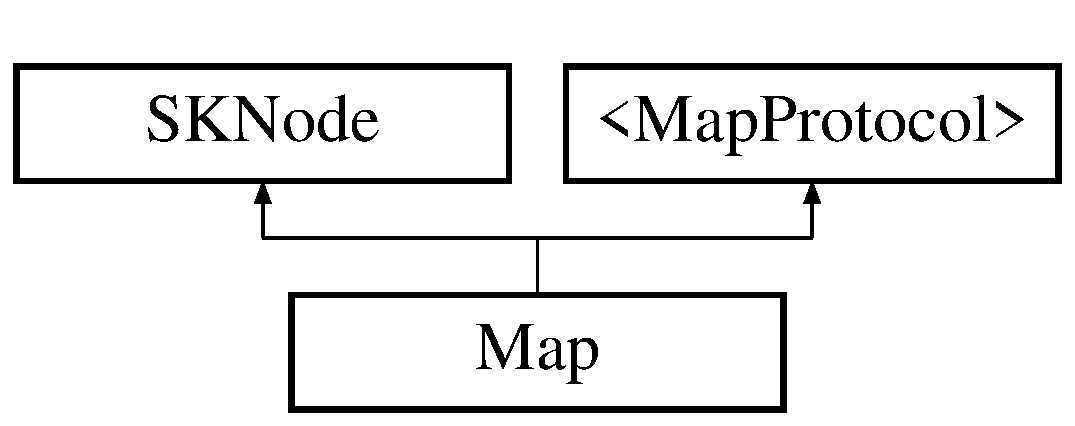
\includegraphics[height=2.000000cm]{interface_map}
\end{center}
\end{figure}
\subsection*{Instance Methods}
\begin{DoxyCompactItemize}
\item 
\hypertarget{interface_map_a008a89cb173753d6425e606ef5e88d73}{(S\+K\+Node $\ast$) -\/ {\bfseries init\+With\+Size\+:}}\label{interface_map_a008a89cb173753d6425e606ef5e88d73}

\item 
\hypertarget{interface_map_a83cc2dc7c5734eb3bda48e99fc15beaf}{(B\+O\+O\+L) -\/ {\bfseries should\+Release\+:}}\label{interface_map_a83cc2dc7c5734eb3bda48e99fc15beaf}

\item 
\hypertarget{interface_map_ab8996e299ab746d6ca386a1f6ca183dc}{(int) -\/ {\bfseries get\+Ball\+Size\+For\+Map}}\label{interface_map_ab8996e299ab746d6ca386a1f6ca183dc}

\item 
\hypertarget{interface_map_a6147f3c603d1ca4ebd47d49c54f28704}{(S\+K\+Shape\+Node $\ast$) -\/ {\bfseries create\+Ball\+With\+Position\+:}}\label{interface_map_a6147f3c603d1ca4ebd47d49c54f28704}

\item 
\hypertarget{interface_map_a6f4bef62fcfa210922cd63e0ef15c927}{(C\+G\+Rect) -\/ {\bfseries area\+For\+Player\+Nr\+:}}\label{interface_map_a6f4bef62fcfa210922cd63e0ef15c927}

\item 
\hypertarget{interface_map_a839f719e4ad796c1c221cd1f90b9de34}{(C\+G\+Point) -\/ {\bfseries start\+Point\+For\+Player\+Nr\+:}}\label{interface_map_a839f719e4ad796c1c221cd1f90b9de34}

\item 
\hypertarget{interface_map_a84bdda86845b75f2d1d8ced7d39a7dfe}{(U\+I\+Color $\ast$) -\/ {\bfseries color\+For\+Player\+Nr\+:}}\label{interface_map_a84bdda86845b75f2d1d8ced7d39a7dfe}

\end{DoxyCompactItemize}
\subsection*{Properties}
\begin{DoxyCompactItemize}
\item 
\hypertarget{interface_map_a8a9dedf353399bbcb9f1d0df8a639c5f}{U\+I\+Bezier\+Path $\ast$ {\bfseries restricted\+Area}}\label{interface_map_a8a9dedf353399bbcb9f1d0df8a639c5f}

\end{DoxyCompactItemize}


The documentation for this class was generated from the following files\+:\begin{DoxyCompactItemize}
\item 
Centeye/Map.\+h\item 
Centeye/Map.\+m\end{DoxyCompactItemize}

\hypertarget{category_map_07_08}{\section{Map() Category Reference}
\label{category_map_07_08}\index{Map()@{Map()}}
}
\subsection*{Properties}
\begin{DoxyCompactItemize}
\item 
\hypertarget{category_map_07_08_a4c47b3798f946da043b58aae7438364a}{C\+G\+Size {\bfseries view\+Size}}\label{category_map_07_08_a4c47b3798f946da043b58aae7438364a}

\item 
\hypertarget{category_map_07_08_a05558c552bf40d6b508b8e6d5af59651}{N\+S\+Mutable\+Array $\ast$ {\bfseries play\+Corner}}\label{category_map_07_08_a05558c552bf40d6b508b8e6d5af59651}

\item 
\hypertarget{category_map_07_08_aae0c38f9dc944d5f71d157316734e893}{N\+S\+Mutable\+Dictionary $\ast$ {\bfseries point\+Areas}}\label{category_map_07_08_aae0c38f9dc944d5f71d157316734e893}

\item 
\hypertarget{category_map_07_08_a7c35b54fd861225f38f607d0e2122622}{N\+S\+Array $\ast$ {\bfseries area\+For\+Player}}\label{category_map_07_08_a7c35b54fd861225f38f607d0e2122622}

\item 
\hypertarget{category_map_07_08_a1414f22a6bebb1662a2223cce2fb23b2}{N\+S\+Array $\ast$ {\bfseries start\+Point\+For\+Player}}\label{category_map_07_08_a1414f22a6bebb1662a2223cce2fb23b2}

\item 
\hypertarget{category_map_07_08_a0da0b33712125f1ecfc566918ae56a1c}{N\+S\+Array $\ast$ {\bfseries color\+For\+Player}}\label{category_map_07_08_a0da0b33712125f1ecfc566918ae56a1c}

\end{DoxyCompactItemize}


The documentation for this category was generated from the following file\+:\begin{DoxyCompactItemize}
\item 
Centeye/Map.\+m\end{DoxyCompactItemize}

\hypertarget{interface_menu}{\section{Menu Class Reference}
\label{interface_menu}\index{Menu@{Menu}}
}
Inheritance diagram for Menu\+:\begin{figure}[H]
\begin{center}
\leavevmode
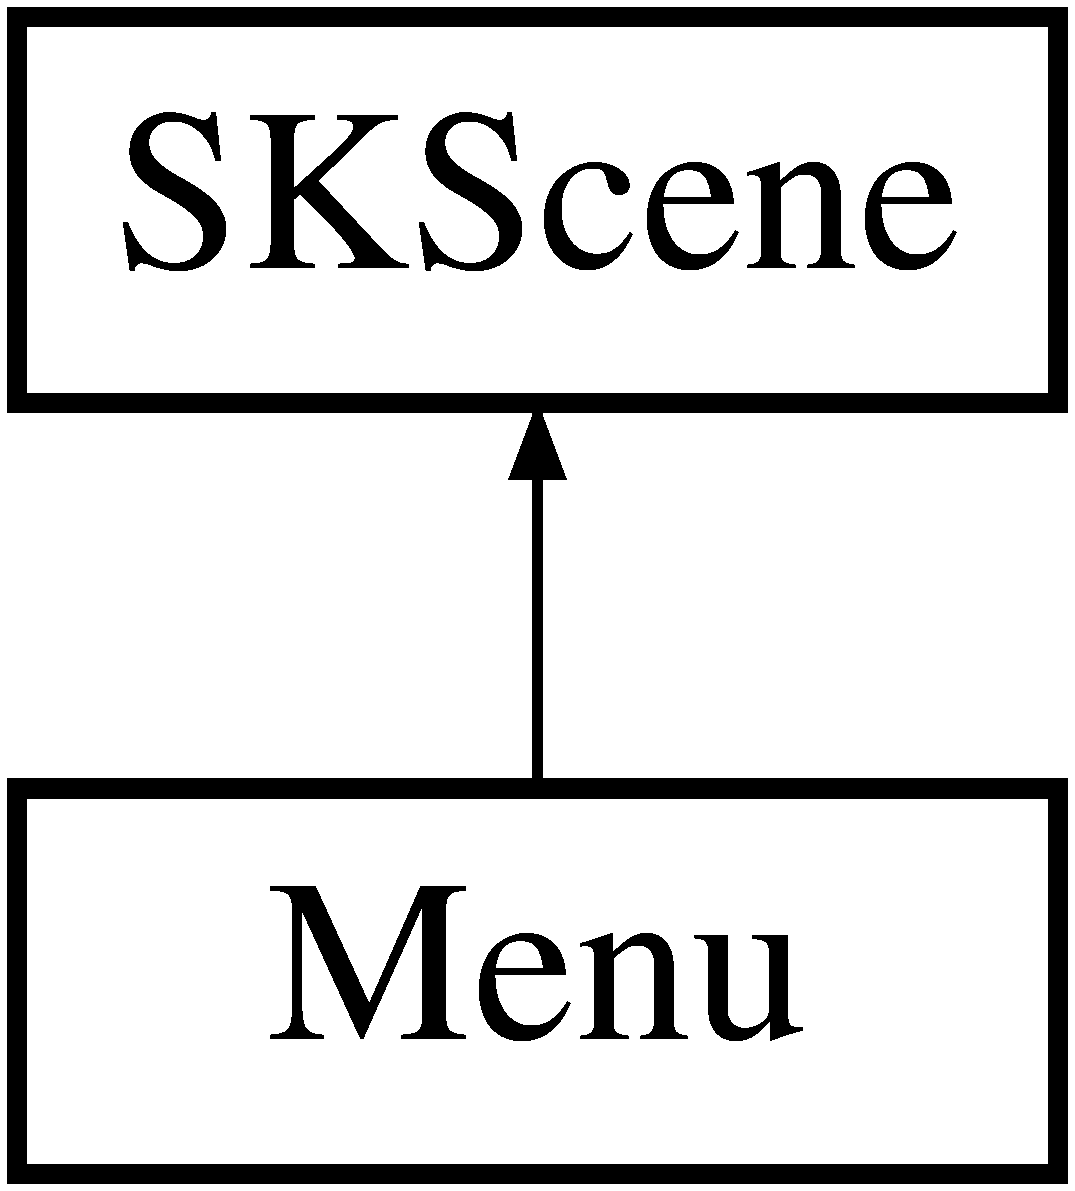
\includegraphics[height=2.000000cm]{interface_menu}
\end{center}
\end{figure}


The documentation for this class was generated from the following file\+:\begin{DoxyCompactItemize}
\item 
Centeye/Menu.\+h\end{DoxyCompactItemize}

\hypertarget{category_menu_07_08}{\section{Menu() Category Reference}
\label{category_menu_07_08}\index{Menu()@{Menu()}}
}
\subsection*{Properties}
\begin{DoxyCompactItemize}
\item 
\hypertarget{category_menu_07_08_a84cf7df2b70e4eee6af3643e20e2bc78}{U\+I\+Tap\+Gesture\+Recognizer $\ast$ {\bfseries gesture\+Recognizer}}\label{category_menu_07_08_a84cf7df2b70e4eee6af3643e20e2bc78}

\item 
\hypertarget{category_menu_07_08_a5aca08847fac2ea9c4bdad900297e13f}{\hyperlink{interface_game_settings}{Game\+Settings} $\ast$ {\bfseries game\+Settings}}\label{category_menu_07_08_a5aca08847fac2ea9c4bdad900297e13f}

\end{DoxyCompactItemize}


The documentation for this category was generated from the following file\+:\begin{DoxyCompactItemize}
\item 
Centeye/Menu.\+m\end{DoxyCompactItemize}

\hypertarget{interface_my_scene}{\section{My\+Scene Class Reference}
\label{interface_my_scene}\index{My\+Scene@{My\+Scene}}
}
Inheritance diagram for My\+Scene\+:\begin{figure}[H]
\begin{center}
\leavevmode
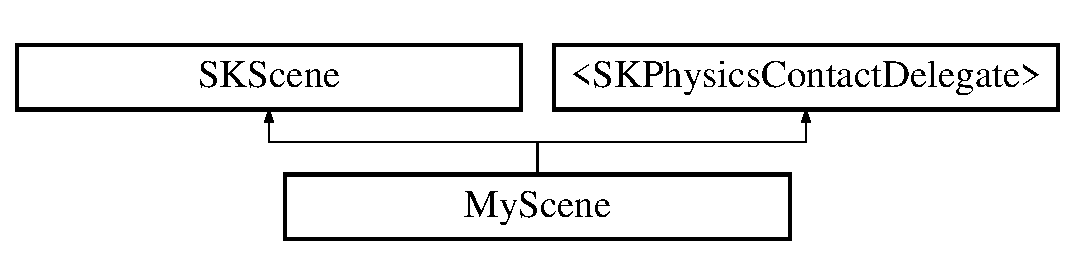
\includegraphics[height=2.000000cm]{interface_my_scene}
\end{center}
\end{figure}


The documentation for this class was generated from the following file\+:\begin{DoxyCompactItemize}
\item 
Centeye/My\+Scene.\+h\end{DoxyCompactItemize}

\hypertarget{category_my_scene_07_08}{\section{My\+Scene() Category Reference}
\label{category_my_scene_07_08}\index{My\+Scene()@{My\+Scene()}}
}
\subsection*{Properties}
\begin{DoxyCompactItemize}
\item 
\hypertarget{category_my_scene_07_08_a3b194a8c83b95893b0e0636a35b71057}{N\+S\+Mutable\+Array $\ast$ {\bfseries players}}\label{category_my_scene_07_08_a3b194a8c83b95893b0e0636a35b71057}

\item 
\hypertarget{category_my_scene_07_08_a5040414971aba6d5589a561648c21bd6}{\hyperlink{interface_map}{Map}$<$ Map\+Protocol $>$ $\ast$ {\bfseries map}}\label{category_my_scene_07_08_a5040414971aba6d5589a561648c21bd6}

\item 
\hypertarget{category_my_scene_07_08_a16e3aa55b0bdb1ced26596c7e4da56b7}{C\+F\+Time\+Interval {\bfseries to\+Next\+Check}}\label{category_my_scene_07_08_a16e3aa55b0bdb1ced26596c7e4da56b7}

\item 
\hypertarget{category_my_scene_07_08_a6be005632b717c9e034cb690d4da197a}{N\+S\+Dictionary $\ast$ {\bfseries point\+Areas}}\label{category_my_scene_07_08_a6be005632b717c9e034cb690d4da197a}

\item 
\hypertarget{category_my_scene_07_08_a162345a329aece9db9d62164104094b8}{int {\bfseries next\+Player\+Id}}\label{category_my_scene_07_08_a162345a329aece9db9d62164104094b8}

\item 
\hypertarget{category_my_scene_07_08_aa5f6554eea28ff36f359b4a7233ce9fc}{B\+O\+O\+L {\bfseries new\+Ball\+Away}}\label{category_my_scene_07_08_aa5f6554eea28ff36f359b4a7233ce9fc}

\item 
\hypertarget{category_my_scene_07_08_a8f9480bf731e872039821063e6df8bd3}{B\+O\+O\+L {\bfseries game\+Over\+Now}}\label{category_my_scene_07_08_a8f9480bf731e872039821063e6df8bd3}

\item 
\hypertarget{category_my_scene_07_08_ad20c1450663f4466f36c270df49d2c05}{\hyperlink{interface_game_settings}{Game\+Settings} $\ast$ {\bfseries game\+Settings}}\label{category_my_scene_07_08_ad20c1450663f4466f36c270df49d2c05}

\item 
\hypertarget{category_my_scene_07_08_aee2276226743e909c9293b4e3860e139}{B\+O\+O\+L {\bfseries score\+Calculated}}\label{category_my_scene_07_08_aee2276226743e909c9293b4e3860e139}

\end{DoxyCompactItemize}


The documentation for this category was generated from the following file\+:\begin{DoxyCompactItemize}
\item 
Centeye/My\+Scene.\+m\end{DoxyCompactItemize}

\hypertarget{interface_player}{\section{Player Class Reference}
\label{interface_player}\index{Player@{Player}}
}
Inheritance diagram for Player\+:\begin{figure}[H]
\begin{center}
\leavevmode
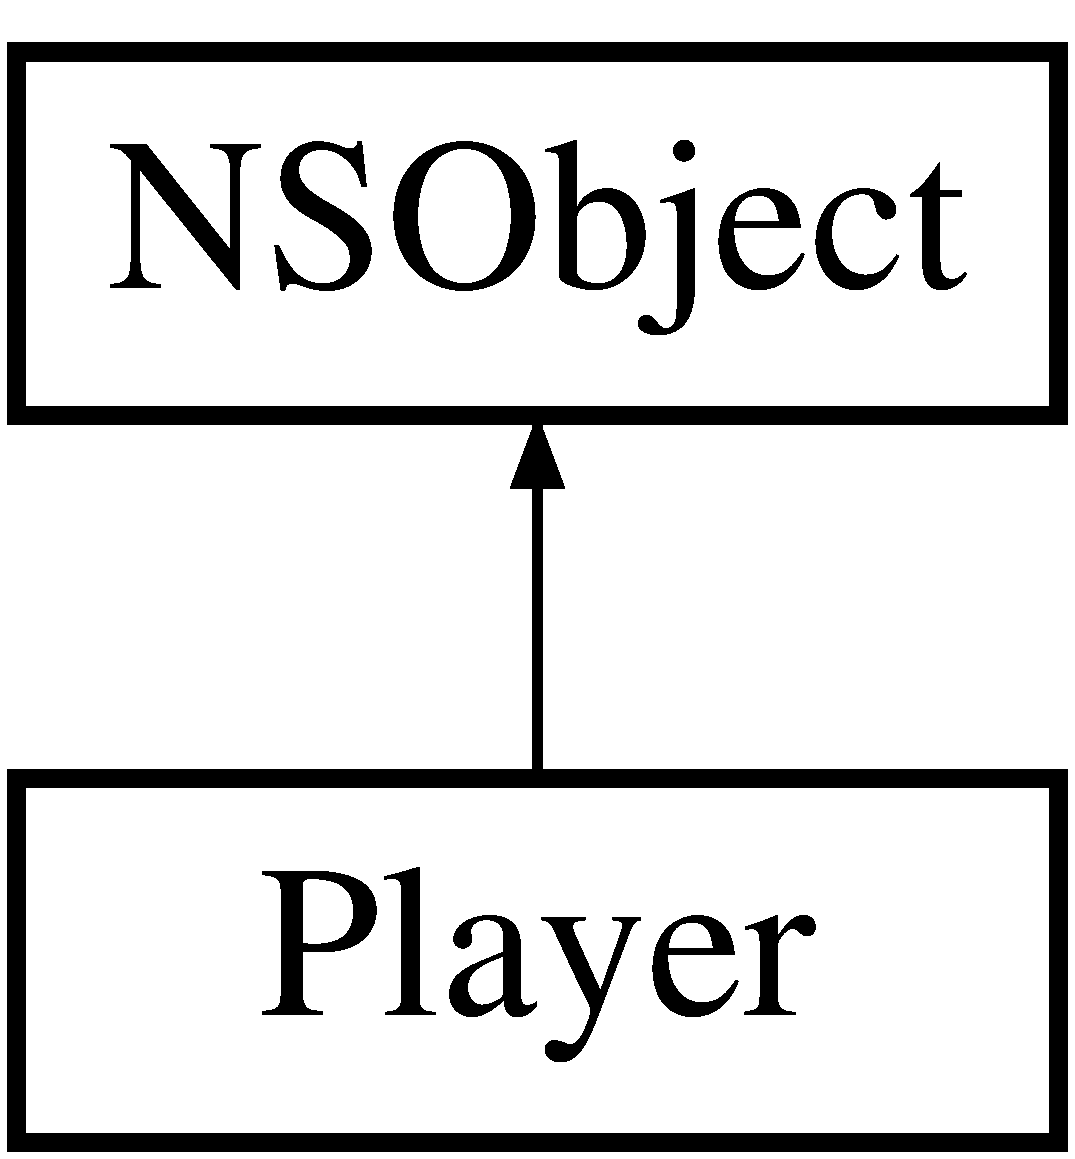
\includegraphics[height=2.000000cm]{interface_player}
\end{center}
\end{figure}
\subsection*{Instance Methods}
\begin{DoxyCompactItemize}
\item 
\hypertarget{interface_player_a3ad0238dee82501d50b26976af25a372}{(\hyperlink{interface_player}{Player} $\ast$) -\/ {\bfseries init\+With\+Color\+:balls\+:}}\label{interface_player_a3ad0238dee82501d50b26976af25a372}

\item 
\hypertarget{interface_player_ac2b67cefe76bf58566a6b2a3bfa7f974}{(B\+O\+O\+L) -\/ {\bfseries has\+Active\+Ball}}\label{interface_player_ac2b67cefe76bf58566a6b2a3bfa7f974}

\item 
\hypertarget{interface_player_aea2eb898f146a2240c48b68b5fadf8d0}{(B\+O\+O\+L) -\/ {\bfseries has\+Balls}}\label{interface_player_aea2eb898f146a2240c48b68b5fadf8d0}

\item 
\hypertarget{interface_player_a1f8c038eddf41a5e1820f82bb1fb0b94}{(B\+O\+O\+L) -\/ {\bfseries is\+In\+Area\+:}}\label{interface_player_a1f8c038eddf41a5e1820f82bb1fb0b94}

\item 
\hypertarget{interface_player_a094a09ea2b78110d213c5543b399e038}{(void) -\/ {\bfseries deactivate\+Ball}}\label{interface_player_a094a09ea2b78110d213c5543b399e038}

\item 
\hypertarget{interface_player_ac23d4de00d9e413375910ca51130626a}{(void) -\/ {\bfseries activate\+Ball\+:}}\label{interface_player_ac23d4de00d9e413375910ca51130626a}

\item 
\hypertarget{interface_player_a3dc9c77d11b1eeae2bb7e5b4f3dd1c72}{(void) -\/ {\bfseries update\+Delta}}\label{interface_player_a3dc9c77d11b1eeae2bb7e5b4f3dd1c72}

\item 
\hypertarget{interface_player_a59f5c1c4d8c9e610e0169ac300bc4cdc}{(void) -\/ {\bfseries set\+Points\+:}}\label{interface_player_a59f5c1c4d8c9e610e0169ac300bc4cdc}

\item 
\hypertarget{interface_player_ab4a4b32bfc22821d0356bd8cf92ed5b6}{(void) -\/ {\bfseries rotate\+Positions\+:}}\label{interface_player_ab4a4b32bfc22821d0356bd8cf92ed5b6}

\item 
\hypertarget{interface_player_a05ed84672c106922f19508f8167a92a1}{(void) -\/ {\bfseries reset\+Player\+With\+Balls\+:}}\label{interface_player_a05ed84672c106922f19508f8167a92a1}

\end{DoxyCompactItemize}
\subsection*{Properties}
\begin{DoxyCompactItemize}
\item 
\hypertarget{interface_player_a3afd3629208045a2227da9fea33f5d08}{S\+K\+Node $\ast$ {\bfseries active\+Ball}}\label{interface_player_a3afd3629208045a2227da9fea33f5d08}

\item 
\hypertarget{interface_player_a0d3dfe848ed5b712459c95dde5ef907d}{S\+K\+Label\+Node $\ast$ {\bfseries score\+Label}}\label{interface_player_a0d3dfe848ed5b712459c95dde5ef907d}

\item 
\hypertarget{interface_player_a904588ceb60dc5e2d447832223c752d8}{int {\bfseries balls}}\label{interface_player_a904588ceb60dc5e2d447832223c752d8}

\item 
\hypertarget{interface_player_a95a6063bbd5905a69f2a063d786bcee4}{C\+G\+Point {\bfseries old\+Position}}\label{interface_player_a95a6063bbd5905a69f2a063d786bcee4}

\item 
\hypertarget{interface_player_a9b4147947fd1cc4989caab553f52ed9c}{C\+G\+Point {\bfseries old\+Old\+Position}}\label{interface_player_a9b4147947fd1cc4989caab553f52ed9c}

\item 
\hypertarget{interface_player_a69a25573708601011eaf03078ccdf874}{C\+F\+Time\+Interval {\bfseries delta}}\label{interface_player_a69a25573708601011eaf03078ccdf874}

\item 
\hypertarget{interface_player_a7d10dd2cc8c7dab46c8d3d808bcbf612}{C\+F\+Time\+Interval {\bfseries old\+Delta}}\label{interface_player_a7d10dd2cc8c7dab46c8d3d808bcbf612}

\item 
\hypertarget{interface_player_a60692ed88922848587c064f41280da99}{C\+F\+Time\+Interval {\bfseries last\+Time}}\label{interface_player_a60692ed88922848587c064f41280da99}

\item 
\hypertarget{interface_player_a8ee978c492fbe16adc8e1155df9de429}{B\+O\+O\+L {\bfseries holding\+Ball}}\label{interface_player_a8ee978c492fbe16adc8e1155df9de429}

\item 
\hypertarget{interface_player_acd53ea389517240216cefb171e784be1}{N\+S\+Mutable\+Array $\ast$ {\bfseries used\+Balls}}\label{interface_player_acd53ea389517240216cefb171e784be1}

\item 
\hypertarget{interface_player_adf0398ea8c1f29175204508ab642b64e}{int {\bfseries points}}\label{interface_player_adf0398ea8c1f29175204508ab642b64e}

\item 
\hypertarget{interface_player_ab531bfc9b7b57ca22fdb1ea45d5e8697}{\hyperlink{interface_player_positions}{Player\+Positions} $\ast$ {\bfseries player\+Positions}}\label{interface_player_ab531bfc9b7b57ca22fdb1ea45d5e8697}

\end{DoxyCompactItemize}


The documentation for this class was generated from the following files\+:\begin{DoxyCompactItemize}
\item 
Centeye/Player.\+h\item 
Centeye/Player.\+m\end{DoxyCompactItemize}

\hypertarget{category_player_07_08}{\section{Player() Category Reference}
\label{category_player_07_08}\index{Player()@{Player()}}
}
\subsection*{Properties}
\begin{DoxyCompactItemize}
\item 
\hypertarget{category_player_07_08_a9b4c91ac2293ba9395a928ffe716bf93}{U\+I\+Color $\ast$ {\bfseries color}}\label{category_player_07_08_a9b4c91ac2293ba9395a928ffe716bf93}

\end{DoxyCompactItemize}


The documentation for this category was generated from the following file\+:\begin{DoxyCompactItemize}
\item 
Centeye/Player.\+m\end{DoxyCompactItemize}

\hypertarget{interface_player_positions}{\section{Player\+Positions Class Reference}
\label{interface_player_positions}\index{Player\+Positions@{Player\+Positions}}
}
Inheritance diagram for Player\+Positions\+:\begin{figure}[H]
\begin{center}
\leavevmode
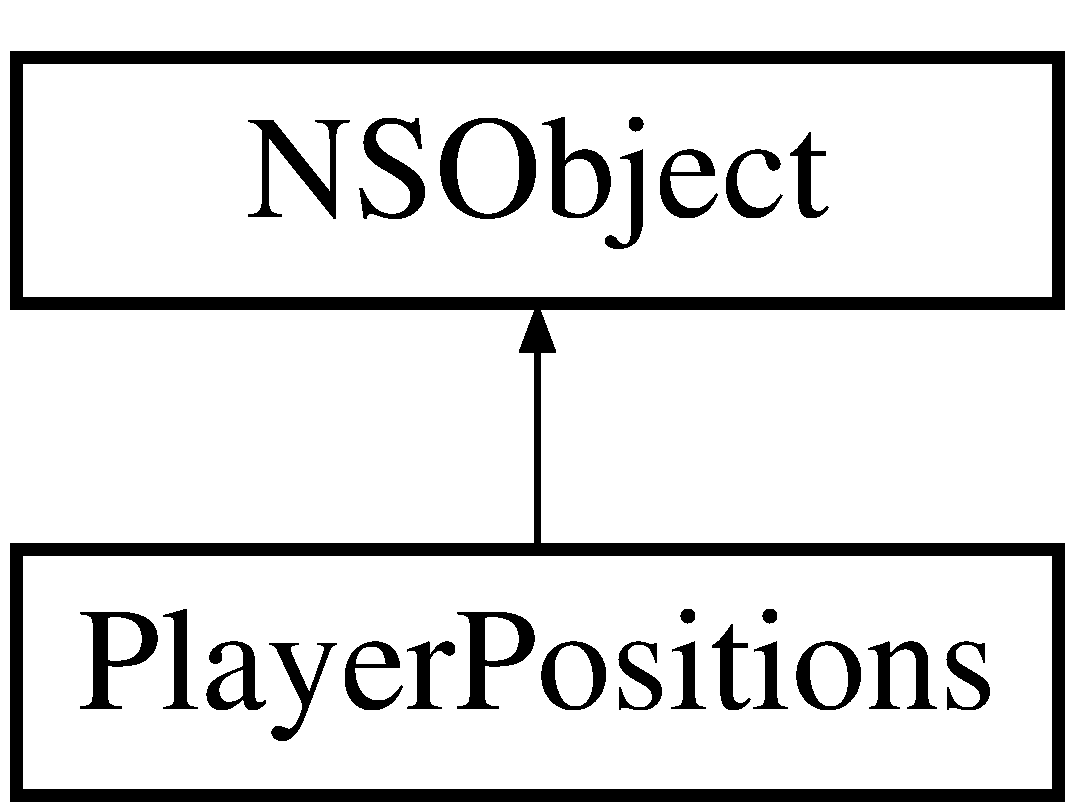
\includegraphics[height=2.000000cm]{interface_player_positions}
\end{center}
\end{figure}
\subsection*{Instance Methods}
\begin{DoxyCompactItemize}
\item 
\hypertarget{interface_player_positions_ac42b194b23965031cf1a0ba992629c73}{(id) -\/ {\bfseries init\+With\+Player\+Nr\+:on\+View\+Size\+:}}\label{interface_player_positions_ac42b194b23965031cf1a0ba992629c73}

\end{DoxyCompactItemize}
\subsection*{Properties}
\begin{DoxyCompactItemize}
\item 
\hypertarget{interface_player_positions_a4aa066ec1cd2887724af7d1123091174}{C\+G\+Point {\bfseries ball\+Start\+Point}}\label{interface_player_positions_a4aa066ec1cd2887724af7d1123091174}

\item 
\hypertarget{interface_player_positions_a816ba5499779e627f95465ee00676ca7}{C\+G\+Rect {\bfseries player\+Area}}\label{interface_player_positions_a816ba5499779e627f95465ee00676ca7}

\item 
\hypertarget{interface_player_positions_aa399c60c9f9cccf608d5473790c96c53}{C\+G\+Point {\bfseries score\+Label\+Point}}\label{interface_player_positions_aa399c60c9f9cccf608d5473790c96c53}

\item 
\hypertarget{interface_player_positions_a37de1ce3fe1539c58ccb1b8193d7d923}{C\+G\+Point {\bfseries ball\+Count\+Point}}\label{interface_player_positions_a37de1ce3fe1539c58ccb1b8193d7d923}

\item 
\hypertarget{interface_player_positions_a02518a6ca7cd3d669f75262530745be6}{C\+G\+Point {\bfseries size\+Up\+Button\+Point}}\label{interface_player_positions_a02518a6ca7cd3d669f75262530745be6}

\item 
\hypertarget{interface_player_positions_a26c381d8943947e24e03e9ee46037d8c}{double {\bfseries score\+Label\+Angle}}\label{interface_player_positions_a26c381d8943947e24e03e9ee46037d8c}

\end{DoxyCompactItemize}


The documentation for this class was generated from the following file\+:\begin{DoxyCompactItemize}
\item 
Centeye/Player\+Positions.\+h\end{DoxyCompactItemize}

\hypertarget{interface_view_controller}{\section{View\+Controller Class Reference}
\label{interface_view_controller}\index{View\+Controller@{View\+Controller}}
}
Inheritance diagram for View\+Controller\+:\begin{figure}[H]
\begin{center}
\leavevmode
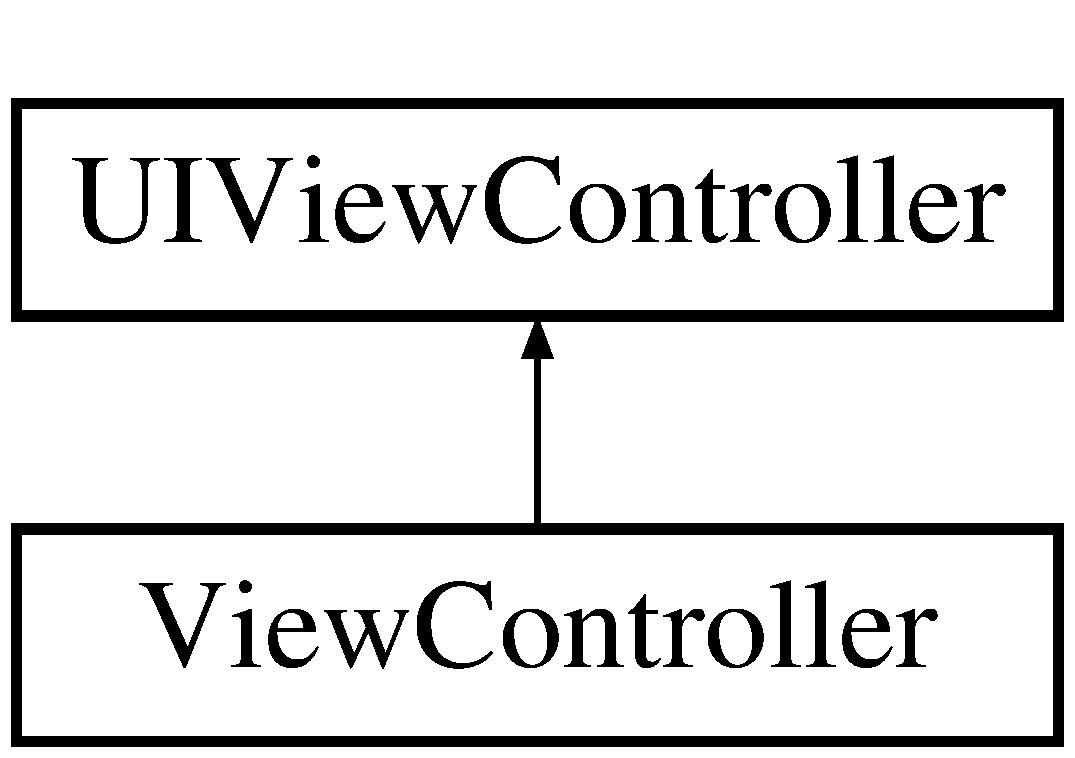
\includegraphics[height=2.000000cm]{interface_view_controller}
\end{center}
\end{figure}


The documentation for this class was generated from the following file\+:\begin{DoxyCompactItemize}
\item 
Centeye/View\+Controller.\+h\end{DoxyCompactItemize}

\hypertarget{category_view_controller_07_08}{\section{View\+Controller() Category Reference}
\label{category_view_controller_07_08}\index{View\+Controller()@{View\+Controller()}}
}
\subsection*{Properties}
\begin{DoxyCompactItemize}
\item 
\hypertarget{category_view_controller_07_08_ab14ebfd1836c1c5803d577e1167e2ac4}{B\+O\+O\+L {\bfseries loaded}}\label{category_view_controller_07_08_ab14ebfd1836c1c5803d577e1167e2ac4}

\end{DoxyCompactItemize}


The documentation for this category was generated from the following file\+:\begin{DoxyCompactItemize}
\item 
Centeye/View\+Controller.\+m\end{DoxyCompactItemize}

%--- End generated contents ---

% Index
\newpage
\phantomsection
\addcontentsline{toc}{chapter}{Index}
\printindex

\end{document}
